\documentclass{minimal}
\usepackage{tikz}
\usepackage{palatino}
\renewcommand{\familydefault}{\sfdefault}

\usetikzlibrary{calc,trees,positioning,arrows,chains,shapes.geometric,%
decorations.pathreplacing,decorations.pathmorphing,shapes,%
matrix,shapes.symbols}

\tikzset{
>=stealth',
punktchain/.style={ rectangle, rounded corners, draw=black, very thick, text width=10em, minimum height=3em, text centered, on chain},
statement/.style={ circle, draw=black, text width=0em, minimum height=0em, text centered},
line/.style={draw, thick, ->},
merge/.style={draw, thick, -},
element/.style={ tape, top color=white, bottom color=blue!50!black!60!, minimum width=8em, draw=blue!40!black!90, very thick, text width=10em, minimum height=3.5em, text centered, on chain},
every join/.style={->, thick,shorten >=1pt},
decoration={brace},
tuborg/.style={decorate},
tubnode/.style={midway, right=2pt, text width=6cm},
}
\begin{document}
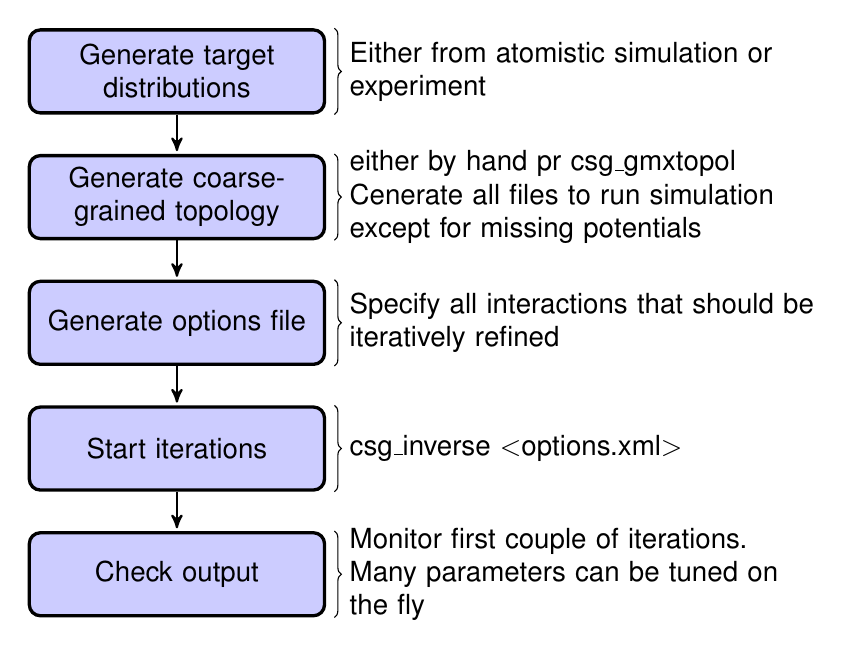
\begin{tikzpicture}
[node distance=.5cm, start chain=going below,]

\node[punktchain, join, fill=blue!20] (ref) {Generate target distributions};
\draw[tuborg, decoration={brace}] let \p1=(ref.north), \p2=(ref.south) in
($(2, \y1)$) -- ($(2, \y2)$) node[tubnode] {Either from atomistic simulation or experiment};

\node[punktchain, join, fill=blue!20] (topol) {Generate coarse-grained topology};
\draw[tuborg, decoration={brace}] let \p1=(topol.north), \p2=(topol.south) in ($(2, \y1)$) -- ($(2, \y2)$) node[tubnode] {either by hand pr csg\_gmxtopol\\Cenerate all files to run simulation except for missing potentials};

\node[punktchain, join, fill=blue!20] (input) {Generate options file};
\draw[tuborg, decoration={brace}] let \p1=(input.north), \p2=(input.south) in ($(2, \y1)$) -- ($(2, \y2)$) node[tubnode] {Specify all interactions that should be iteratively refined};

\node[punktchain, join, fill=blue!20] (ibi) {Start iterations};
\draw[tuborg, decoration={brace}] let \p1=(ibi.north), \p2=(ibi.south) in ($(2, \y1)$) -- ($(2, \y2)$) node[tubnode] {csg\_inverse $<$options.xml$>$};

\node[punktchain, join, fill=blue!20] (check) {Check output};
\draw[tuborg, decoration={brace}] let \p1=(check.north), \p2=(check.south) in ($(2, \y1)$) -- ($(2, \y2)$) node[tubnode] {Monitor first couple of iterations.\\Many parameters can be tuned on the fly};

\end{tikzpicture}
\end{document}
